\documentclass[tikz,border=8pt]{standalone}
% Shared look for every TikZ diagram. Load with \input{../../tools/tikz-style.tex}
\usepackage[T1]{fontenc}
\usepackage{lmodern}
\renewcommand{\sfdefault}{lmr}  % diagrams use the same serif as the text
\usetikzlibrary{arrows.meta, positioning, shapes.geometric, calc, fit, backgrounds}
\definecolor{cblue}{HTML}{4C78A8}
\definecolor{corange}{HTML}{F58518}
\definecolor{cgreen}{HTML}{54A24B}
\definecolor{cred}{HTML}{E45756}
\definecolor{cpurple}{HTML}{B279A2}
\definecolor{cgrey}{HTML}{6B6B6B}
\tikzset{
  every picture/.style={font=\sffamily, line width=1.2pt},
  box/.style={draw=#1, fill=#1!12, rounded corners=4pt, align=center, inner sep=7pt, minimum height=1.1cm},
  box/.default=cgrey,
  arrow/.style={-{Stealth[length=3mm]}, draw=cgrey, line width=1.4pt},
  title/.style={font=\sffamily\bfseries\Large},
  note/.style={font=\sffamily\small, text=cgrey, align=center},
}
\AtBeginDocument{\hyphenpenalty=10000 \exhyphenpenalty=10000}

\begin{document}
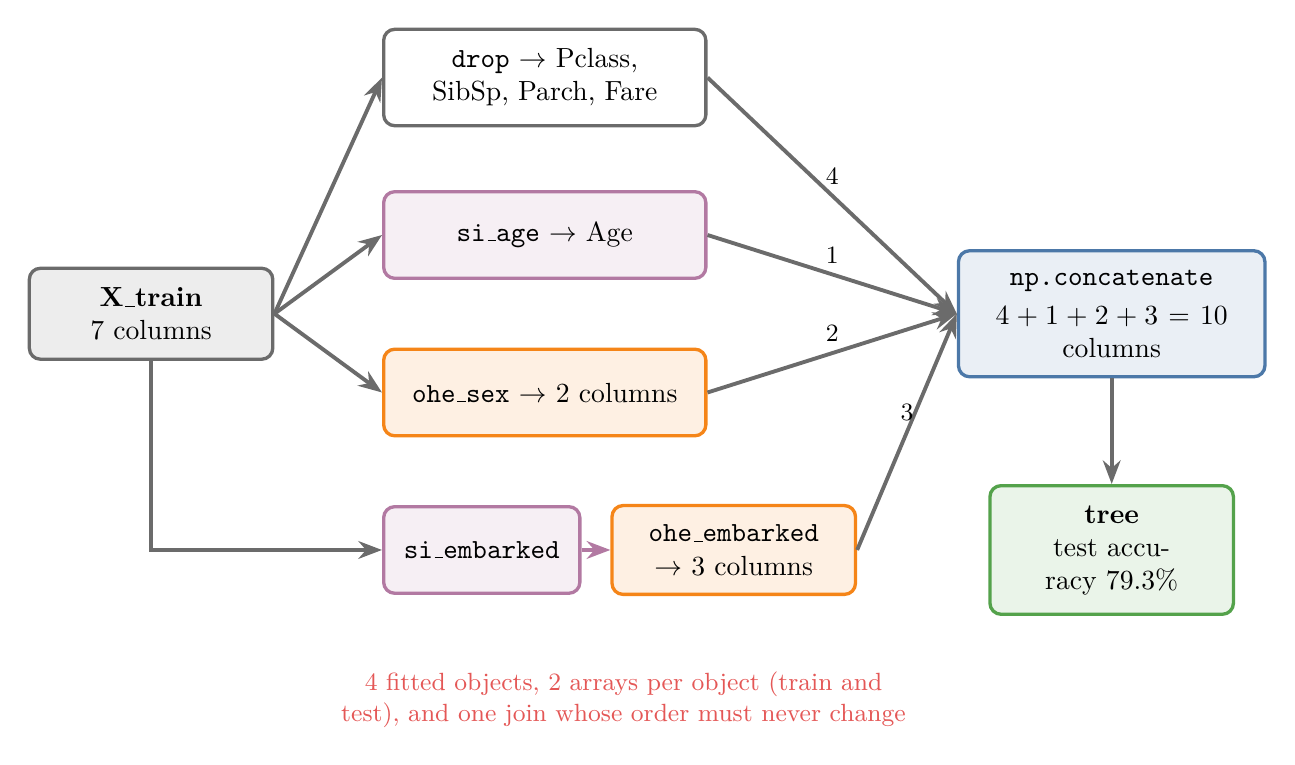
\begin{tikzpicture}
  \node[box=cgrey, text width=2.6cm] (x) at (0,0) {\textbf{X\_train}\\7 columns};
  \node[box=cgrey, fill=white, text width=3.6cm] (rem) at (5,3) {\texttt{drop} $\to$ Pclass, SibSp, Parch, Fare};
  \node[box=cpurple, text width=3.6cm] (age) at (5,1) {\texttt{si\_age} $\to$ Age};
  \node[box=corange, text width=3.6cm] (sex) at (5,-1) {\texttt{ohe\_sex} $\to$ 2 columns};
  \node[box=cpurple, text width=2.0cm] (emb1) at (4.2,-3) {\texttt{si\_embarked}};
  \node[box=corange, text width=2.6cm] (emb2) at (7.4,-3) {\texttt{ohe\_embarked} $\to$ 3 columns};
  \draw[arrow, draw=cpurple] (emb1) -- (emb2);
  \foreach \t in {rem, age, sex} \draw[arrow] (x.east) -- (\t.west);
  \draw[arrow] (x.south) |- (emb1.west);
  \node[box=cblue, text width=3.4cm] (cat) at (12.2,0) {\texttt{np.concatenate}\\[2pt] $4 + 1 + 2 + 3 = 10$ columns};
  \foreach \t/\n in {rem/4, age/1, sex/2, emb2/3} \draw[arrow] (\t.east) -- node[above, font=\small] {\n} (cat.west);
  \node[box=cgreen, text width=2.6cm] (clf) at (12.2,-3) {\textbf{tree}\\test accuracy 79.3\%};
  \draw[arrow] (cat) -- (clf);
  \node[note, text=cred, text width=11cm] at (6,-4.9) {4 fitted objects, 2 arrays per object (train and test), and one join whose order must never change};
\end{tikzpicture}
\end{document}
